\documentclass[a4paper, 11pt]{article}
\usepackage[top=3cm, bottom=3cm, left = 2cm, right = 2cm]{geometry}
\usepackage[brazilian]{babel}
\usepackage{setspace}
\usepackage{graphicx}
\usepackage{mwe}
\usepackage{float}
\usepackage{chngcntr}

\title{Relatório: Trabalho 2 -- Otimização de Desempenho}
\author{Gabriel Lisboa Conegero -- GRR20221255\\
Pedro Folloni Pesserl -- GRR20220072\\
\textit{Departamento de Informática}\\
\textit{Universidade Federal do Paraná -- UFPR}\\
Curitiba, Brasil\\
\texttt{glc22@inf.ufpr.br, pfp22@inf.ufpr.br}}
\date{}

\begin{document}
\maketitle

\begin{abstract}
\begin{singlespace}
    Este relatório documenta o processo de otimização de um programa que
    realiza ajuste polinomial de curvas, utilizando o método dos
    \textbf{Mínimos Quadrados} e \textbf{Eliminação de Gauss}. Também
    apresenta a comparação entre as duas versões do programa, obtida a
    partir da ferramenta LIKWID.
\end{singlespace}
\end{abstract}

\section{Metodologia da análise}
A análise do programa de ajuste polinomial de curvas foi feita considerando
três seções principais do código, que realizam, respectivamente:
\begin{enumerate}
    \item Geração do sistema linear pelo método dos Mínimos Quadrados;
    \item Solução do sistema linear pelo método da Eliminação de Gauss;
    \item Cálculo de resíduos do polinômio encontrado.
\end{enumerate}
Tanto a seção de geração do sistema linear quanto a de cálculo dos resíduos do
polinômio foram avaliadas com as seguintes métricas: tempo de execução, número
de operações aritméticas de ponto flutuante por segundo (FLOP/s), com e sem uso
de SIMD, banda de memória utilizada e taxa de \textit{miss} na \textit{cache}
de dados. A seção de solução do sistema linear teve seu desempenho avaliado em
tempo de execução e FLOP/s, apenas.

\section{Otimizações realizadas}
\subsection{Geração do sistema linear}
\label{subsection:gera_sl}
Originalmente, a versão 1 do programa utilizava uma tabela de \textit{lookup}
para armazenar as potências, de 0 a $2m$, dos pontos de entrada, onde $m$ é o
grau do polinômio a ser ajustado. Porém, isso precisou ser modificado, porque a
entrada agora pode conter até $10^8$ pontos, o que impossibilita o
armazenamento das potências de todos os pontos na memória. Então, a versão 1
agora utiliza a função \texttt{pow\_inter()} para calcular as potências dos
$x$'s a cada iteração.

A otimização empregada na versão 2 foi inverter a ordem dos laços no cálculo
das potências, de forma que iteramos sobre o vetor de pontos de entrada apenas
uma vez, possibilitando que ele seja mantido (ainda que em parte) em
\textit{cache}. Dessa maneira, percorremos a primeira linha e última coluna da
matriz do sistema linear e o vetor de termos independentes múltiplas vezes,
calculando a próxima potência do ponto atual que estamos somando a cada
iteração com apenas uma multiplicação sobre a potência anterior.

Como o vetor de pontos é muito maior do que a matriz do sistema linear, que é
sempre de ordem 5, espera-se que isso diminua a taxa de \textit{miss} na
\textit{cache} por ser necessário recarregá-lo em \textit{cache} menos vezes.

\subsection{Cálculo de resíduos}
Pela mesma questão apresentada na subseção \ref{subsection:gera_sl}, a versão
1 do programa foi modificada para usar a função \texttt{pow\_inter()} na
computação das potências dos pontos de entrada, para que fossem aplicadas no
cálculo do polinômio com os coeficientes encontrados.

A versão 2 utiliza a mesma estratégia de multiplicar iterativamente cada $x_i$
pela potência já calculada na iteração anterior, de forma a substituir a
função custosa \texttt{pow\_inter()} por uma multiplicação a cada passo.

\subsection{Outras}
Além do que já foi mencionado, demais otimizações incluem a criação de uma
estrutura \texttt{struct Ponto\_t}, para que os pontos de entrada fossem
armazenados em um vetor de estruturas em vez de em dois vetores separados.
Essa decisão foi tomada porque sempre que o valor $x$ de um ponto é acessado
no programa, o valor de $y$ correspondente também é usado. Dessa forma, quando
um ponto é usado em algum cálculo, ambas as suas coordenadas já estão carregadas
em \textit{cache}. Essa otimização tem impacto tanto na função que gera o
sistema linear quanto na do cálculo dos resíduos.

Além disso, também foi feita a substituição das funções de manipulação de
intervalos por suas contrapartes \texttt{inline}, o que possibilita o
aproveitamento do \textit{pipeline} do processador por não ser necessário
desviar o fluxo de execução para a área de definição das funções.

\section{Gráficos}
Os gráficos aqui apresentados foram gerados por meio da ferramenta gnuplot.
\def\path{../resultados/graficos}

\counterwithin{figure}{subsection}
\renewcommand{\thefigure}{\arabic{subsection}.\arabic{figure}}

\subsection{Geração do sistema linear}
\label{subsecao:gera_sl}
\begin{figure}[H]
    \centering
    \begin{minipage}{.5\textwidth}
        \centering
        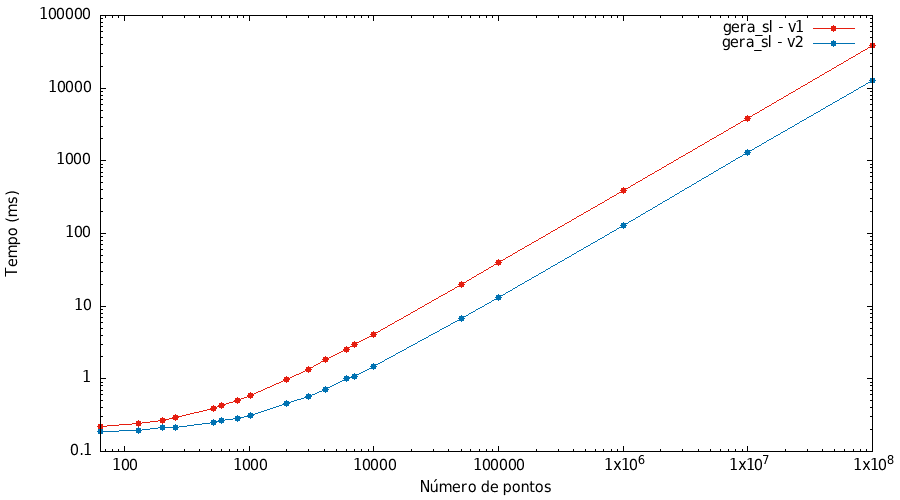
\includegraphics[width=\linewidth]{\path/tempo_gera_sl.png}
        \caption{Tempo de execução.}
        \label{gera_sl:tempo}
    \end{minipage}\hfill
    \begin{minipage}{.5\textwidth}
        \centering
        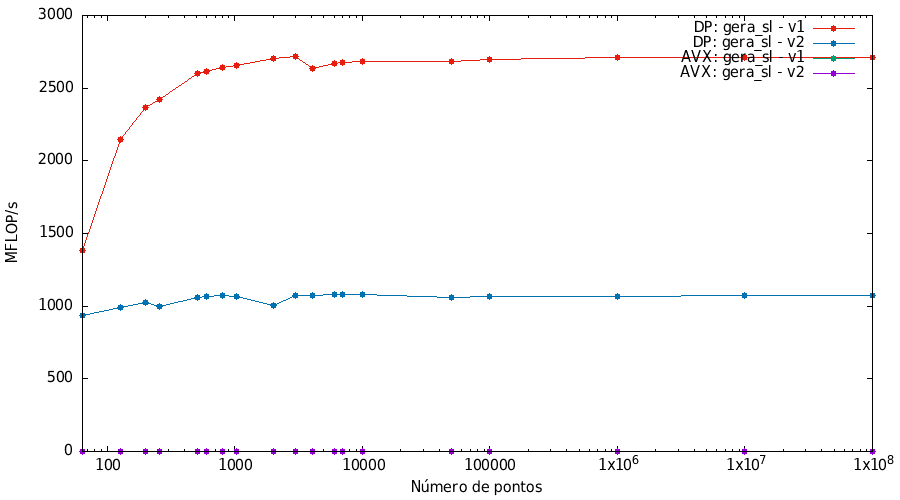
\includegraphics[width=\linewidth]{\path/operacoes_aritmeticas_gera_sl.png}
        \caption{Número de operações de ponto flutuante por segundo.}
        \label{gera_sl:flops}
    \end{minipage}
\end{figure}

Percebe-se pela figura \ref{gera_sl:tempo} uma redução de aproximadamente 4 vezes
no tempo de execução da geração do sistema; isso se deve às otimizações de uso da
\textit{cache} e cálculo das potências dos valores de entrada.

A figura \ref{gera_sl:flops} demonstra que a quantidade de FLOP/s é muito
maior na versão 1, por causa do uso da função \texttt{pow\_inter()}. A versão
2 tem menos FLOP/s devido ao reaproveitamento dos cálculos para exponenciação
do intervalo.

\begin{figure}[H]
    \centering
    \begin{minipage}{.5\textwidth}
        \centering
        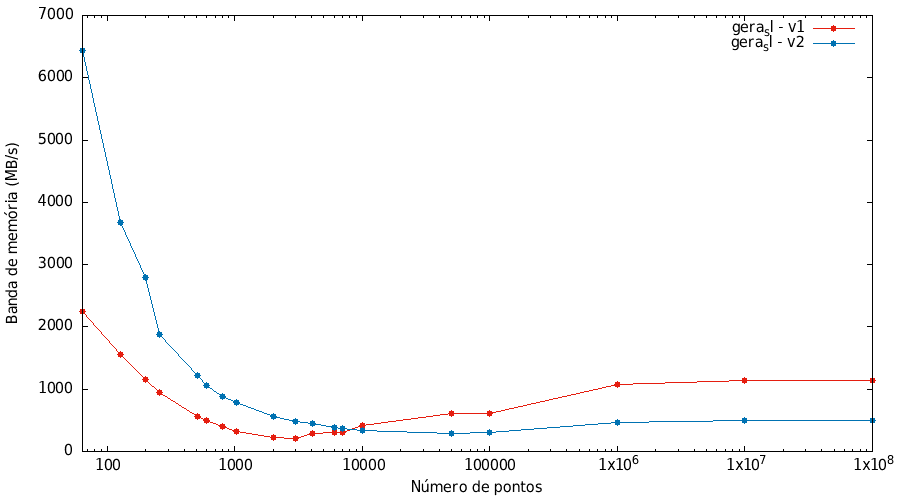
\includegraphics[width=\linewidth]{\path/banda_de_memoria_gera_sl.png}
        \caption{Banda de memória utilizada.}
        \label{gera_sl:banda}
    \end{minipage}\hfill
    \begin{minipage}{.5\textwidth}
        \centering
        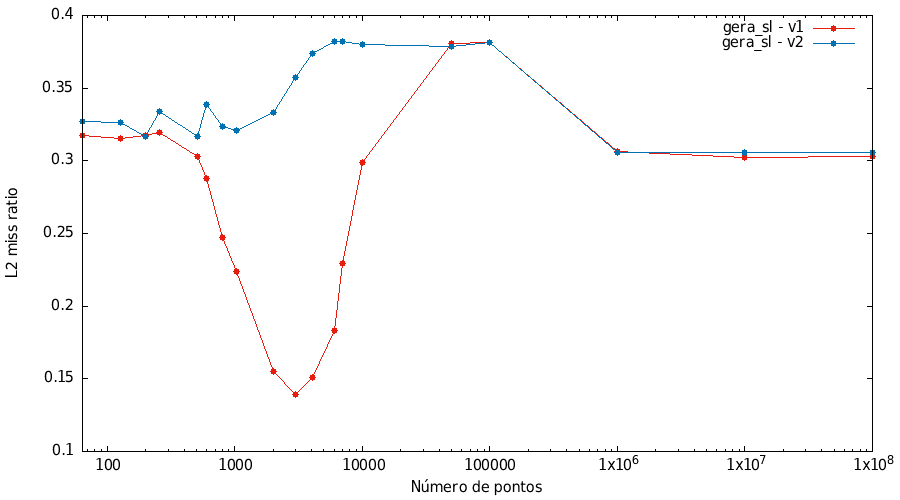
\includegraphics[width=\linewidth]{\path/cache_miss_l2_gera_sl.png}
        \caption{Taxa de \textit{miss} na \textit{cache} L2.}
        \label{gera_sl:cache_miss}
    \end{minipage}
\end{figure}

Como relatado em \ref{gera_sl:banda}, a banda de memória utilizada é cerca de uma
uma ordem de magnitude maior na versão 2, para um número pequeno de pontos. A origem
desse aumento são as otimizações que mantêm os dados na \textit{cache}. Contudo,
conforme o número de pontos aumenta, as taxas vão diminuindo e se igualando, devido
ao aumento de \textit{cache miss}.

O comportamento apresentado na figura \ref{gera_sl:cache_miss} foi inesperado: com
às otimizações de uso da cache, o resultado esperado era que a versão 2 tivesse um
\textit{cache miss} menor que a versão 1.

\subsection{Solução do sistema linear}
\begin{figure}[H]
    \centering
    \begin{minipage}{.5\textwidth}
        \centering
        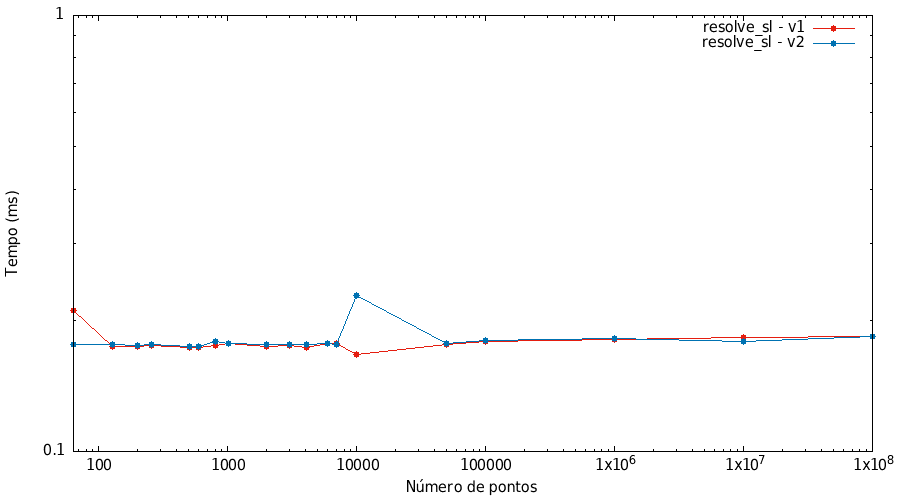
\includegraphics[width=\linewidth]{\path/tempo_resolve_sl.png}
        \caption{Tempo de execução.}
        \label{resolve_sl:tempo}
    \end{minipage}\hfill
    \begin{minipage}{.5\textwidth}
        \centering
        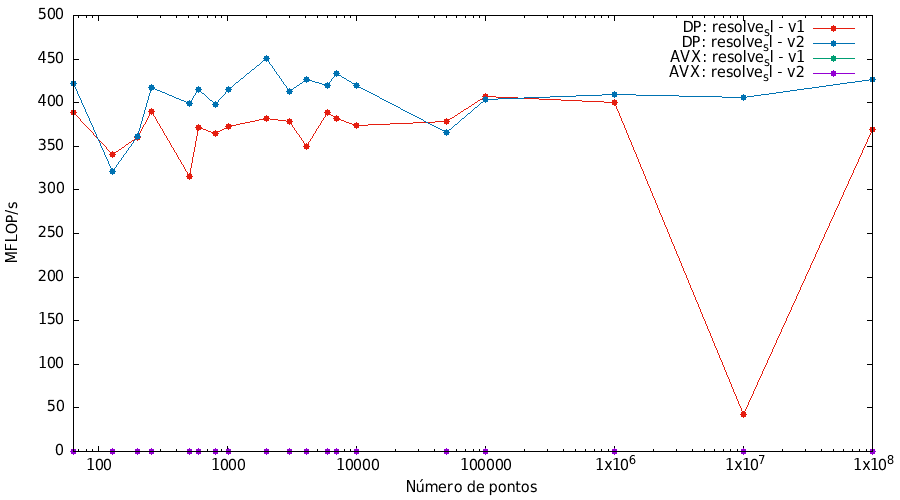
\includegraphics[width=\linewidth]{\path/operacoes_aritmeticas_resolve_sl.png}
        \caption{Número de operações de ponto flutuante por segundo.}
        \label{resolve_sl:flops}
    \end{minipage}
\end{figure}

Percebe-se pela figura \ref{resolve_sl:tempo} que o tempo de execução da
solução do sistema linear foi aproximadamente constante, indepentendemente
do número de pontos da entrada. Isso é devido ao fato de que a matriz sempre
possui ordem 5, e os cálculos não utilizam a função \texttt{pow\_inter()}.

Essa relativa constância se repetiu na análise de FLOP/s, como apresentado na figura
\ref{resolve_sl:flops}, pelos mesmo motivo descritos acima.

\subsection{Cálculo de resíduos}
\begin{figure}[H]
    \centering
    \begin{minipage}{.5\textwidth}
        \centering
        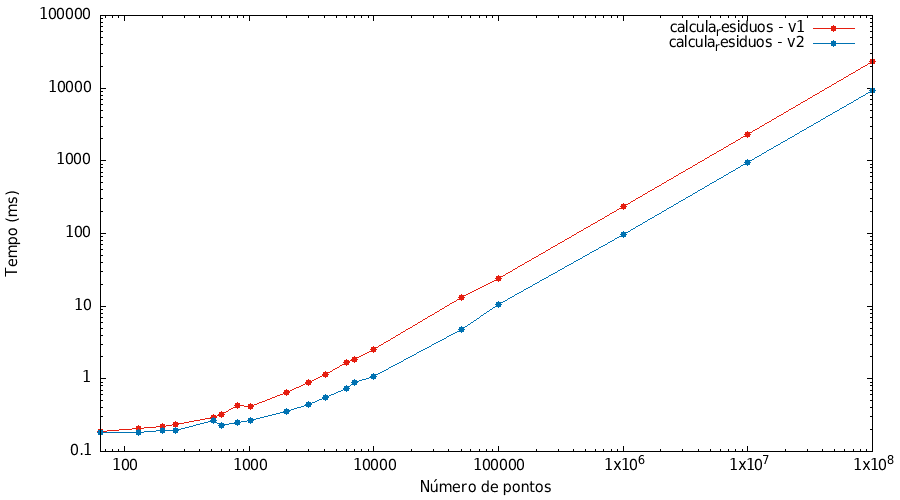
\includegraphics[width=\linewidth]{\path/tempo_calcula_residuos.png}
        \caption{Tempo de execução.}
        \label{calcula_residuos:tempo}
    \end{minipage}\hfill
    \begin{minipage}{.5\textwidth}
        \centering
        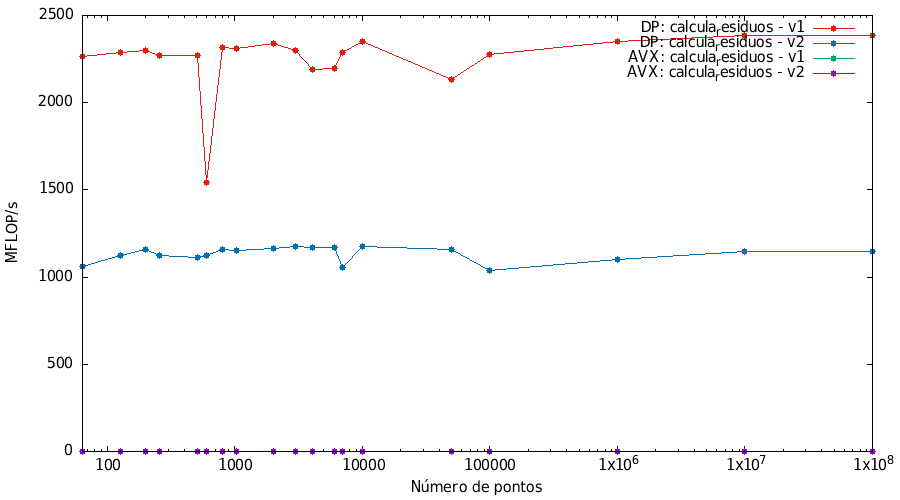
\includegraphics[width=\linewidth]{\path/operacoes_aritmeticas_calcula_residuos.png}
        \caption{Número de operações de ponto flutuante por segundo.}
        \label{calcula_residuos:flops}
    \end{minipage}
\end{figure}

Como na função geradora do sistema linear, é possível perceber pela figura
\ref{calcula_residuos:tempo} que o tempo de execução da função que calcula
resíduos foi reduzido em cerca de 4 vezes. Isso se deve à otimização do uso
da função \texttt{pow\_inter()} e do uso de dados na \textit{cache}.

O número de FLOP/s foi reduzido pela metade na função de cálculo de resíduos,
como apresentado na figura \ref{calcula_residuos:flops}. Isso porque a versão
2 otimiza o código e reaproveita a potência $x_i^k$, calculada em uma iteração,
para calcular a potência $x_i^{k+1}$ na próxima, em lugar de utilizar a função
\texttt{pow\_inter()}.

\begin{figure}[H]
    \centering
    \begin{minipage}{.5\textwidth}
        \centering
        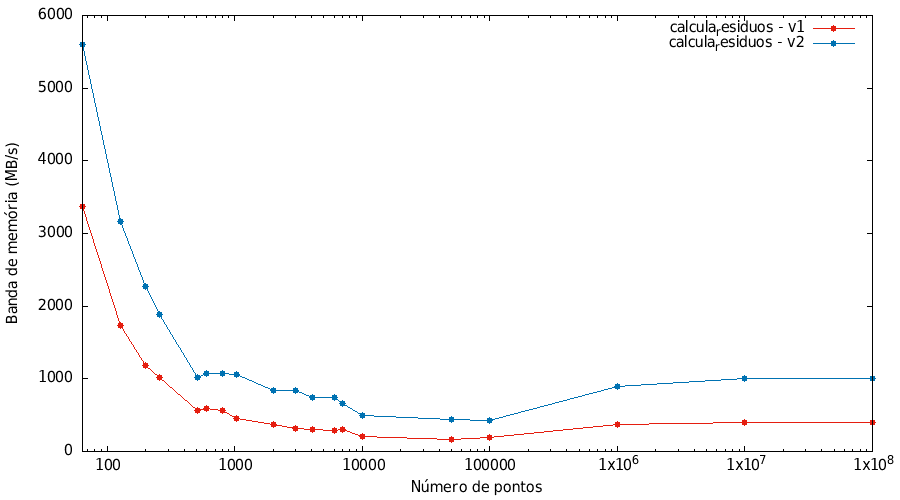
\includegraphics[width=\linewidth]{\path/banda_de_memoria_calcula_residuos.png}
        \caption{Banda de memória utilizada.}
        \label{calcula_residuos:banda}
    \end{minipage}\hfill
    \begin{minipage}{.5\textwidth}
        \centering
        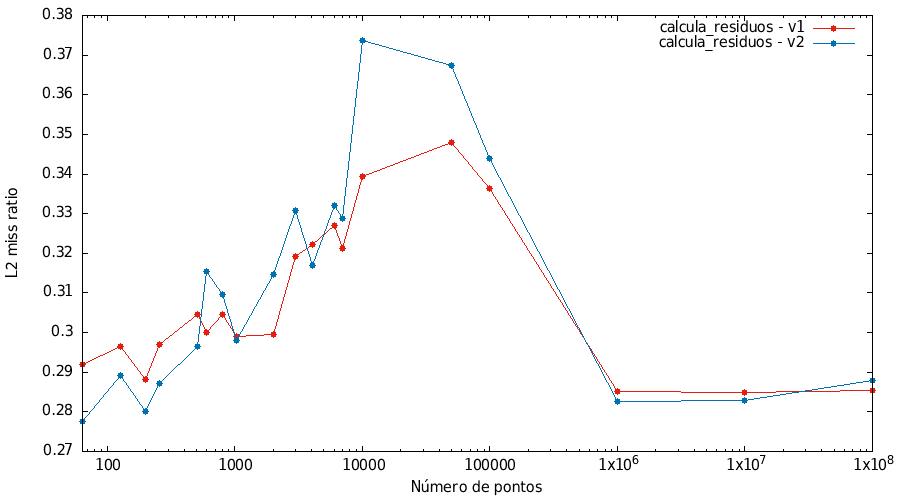
\includegraphics[width=\linewidth]{\path/cache_miss_l2_calcula_residuos.png}
        \caption{Taxa de \textit{miss} na \textit{cache} L2.}
        \label{calcula_residuos:cache_miss}
    \end{minipage}
\end{figure}

Na figura \ref{calcula_residuos:banda}, pode-se perceber que a função usa,
aproximadamente, o dobro de banda de memória na segunda versão quando comparada
com a primeira, por conta das otimizações de cache e CPU mencionadas.

Porém, novamente, constatamos que a taxa de \textit{cache miss} foi aproximadamente
igual ou maior na versão 2 do que na versão 1, como descrito na figura
\ref{calcula_residuos:cache_miss}, que é um resultado inesperado.

\section{Arquitetura do processador utilizado}
    Saída do comando \texttt{likwid-topology -g -c}.
    \begin{verbatim}
--------------------------------------------------------------------------------
CPU name:	Intel(R) Core(TM) i5-7500 CPU @ 3.40GHz
CPU type:	Intel Coffeelake processor
CPU stepping:	9
********************************************************************************
Hardware Thread Topology
********************************************************************************
Sockets:		1
Cores per socket:	4
Threads per core:	1
--------------------------------------------------------------------------------
HWThread	Thread		Core		Socket		Available
0		0		0		0		*
1		0		1		0		*
2		0		2		0		*
3		0		3		0		*
--------------------------------------------------------------------------------
Socket 0:		( 0 1 2 3 )
--------------------------------------------------------------------------------
********************************************************************************
Cache Topology
********************************************************************************
Level:			1
Size:			32 kB
Type:			Data cache
Associativity:		8
Number of sets:		64
Cache line size:	64
Cache type:		Non Inclusive
Shared by threads:	1
Cache groups:		( 0 ) ( 1 ) ( 2 ) ( 3 )
--------------------------------------------------------------------------------
Level:			2
Size:			256 kB
Type:			Unified cache
Associativity:		4
Number of sets:		1024
Cache line size:	64
Cache type:		Non Inclusive
Shared by threads:	1
Cache groups:		( 0 ) ( 1 ) ( 2 ) ( 3 )
--------------------------------------------------------------------------------
Level:			3
Size:			6 MB
Type:			Unified cache
Associativity:		12
Number of sets:		8192
Cache line size:	64
Cache type:		Inclusive
Shared by threads:	4
Cache groups:		( 0 1 2 3 )
--------------------------------------------------------------------------------
********************************************************************************
NUMA Topology
********************************************************************************
NUMA domains:		1
--------------------------------------------------------------------------------
Domain:			0
Processors:		( 0 1 2 3 )
Distances:		10
Free memory:		5171.89 MB
Total memory:		7826.25 MB
--------------------------------------------------------------------------------


********************************************************************************
Graphical Topology
********************************************************************************
Socket 0:
+---------------------------------------------+
| +--------+ +--------+ +--------+ +--------+ |
| |    0   | |    1   | |    2   | |    3   | |
| +--------+ +--------+ +--------+ +--------+ |
| +--------+ +--------+ +--------+ +--------+ |
| |  32 kB | |  32 kB | |  32 kB | |  32 kB | |
| +--------+ +--------+ +--------+ +--------+ |
| +--------+ +--------+ +--------+ +--------+ |
| | 256 kB | | 256 kB | | 256 kB | | 256 kB | |
| +--------+ +--------+ +--------+ +--------+ |
| +-----------------------------------------+ |
| |                   6 MB                  | |
| +-----------------------------------------+ |
+---------------------------------------------+
    \end{verbatim}
\end{document}
